\chapter{编写第一个系统调用}

什么是系统调用?在我们使用C语言编程时,使用过库函数提供的一些基本的函数,例如:控制台输出、文件读写。
我们使用库函数完成基本的操作,库函数是对操作系统提供的系统调用的进一步封装,并隐藏掉了一些操作。
系统调用工作在最底层,使用POSIX提供的接口,直接操作硬件,完成最基本的操作。

为什么需要借助于操作系统,用户不能直接操作硬件呢?
凡是与资源有关的操作、会影响到其它进程的操作,为了方便管理资源(防止恶意操作)、使进程间隔离,
操作系统必须介入,实现统一管理调度。操作系统为上层编程语言提供了一套接口,这套接口就是系统调用。
用户库封装系统调用为库函数还有以下优点:

\textbf{1. 简化用户程序的编写:}通过封装系统调用,用户程序可以使用更为简单和直观的接口来完成复杂的系统操作,
无需了解系统调用的底层细节,减少程序员的开发难度。

\textbf{2. 提高代码的可维护性:}通过库函数的封装,程序员可以对库函数进行多层封装,使程序的可读性、可维护性更高。
当需要进行修改时,只需修改库函数的实现,无需修改应用程序的代码,降低了代码的耦合度,减少了代码维护的成本。

\textbf{3. 提高程序的移植性:}不同的操作系统和硬件平台实现系统调用的方式可能略有不同。
使用库函数来封装系统调用可以提高程序的移植性。如果需要在不同操作系统下运行程序,只需更改库函数的实现即可。

\textbf{4. 方便进行错误处理:}库函数可以对系统调用返回值进行处理,根据返回值不同的情况进行错误处理。
在使用系统调用时,程序员需要手动进行错误处理,使用库函数可以减轻程序员的工作量。

总之,封装系统调用为库函数可以使得程序更加简单、稳定、易维护、易移植,并且可以提高程序员的开发效率。

为了区分一个操作是用户完成的,还是依赖于操作系统完成的,每种指令集体系结构都对此做出了区分。
以RISC-V架构为例,CPU的工作状态分为用户态、内核态等。执行用户程序指令时的状态为用户态,需要发起系统调用时,
库函数中ecall指令会使CPU发生陷入提高特权级,到达内核态。内核态完成操作后,使用ret指令降低特权级,回到用户态。

本章将首先以三个系统调用为例子,讲解在用户态程序中如何使用系统调用,之后使用调试工具跟踪观察系统调用的实现,
最后将对系统调用以及用户态、内核态等展开详细介绍。

\section{使用系统调用}

本节将以三个常见系统调用为例,简要介绍在用户态用户进程是如何使用系统调用的。

\subsection{fork}

fork是一种用于克隆进程的全部内存空间的系统调用,是Linux系统中创建一个新进程的重要方法,除了第一个进程,
所有的进程都是由fork创建的。

这是一个 Rust 语言编写的程序,主要目的是展示如何使用 fork 函数创建子进程,如\autoref{code:forktest}所示。

\begin{lstlisting}[language={Rust}, label={code:forktest},
    caption={forktest.rs}]
#![no_std]
#![no_main]

#[macro_use]
extern crate user_lib;

use user_lib::{exit, fork, wait};

const MAX_CHILD: usize = 30;

#[no_mangle]
pub fn main() -> i32 {
    for i in 0..MAX_CHILD {
        let pid = fork();
        if pid == 0 {
            println!("I am child {}", i);
            exit(0);
        } else {
            println!("forked child pid = {}", pid);
        }
        assert!(pid > 0);
    }
    let mut exit_code: i32 = 0;
    for _ in 0..MAX_CHILD {
        if wait(&mut exit_code) <= 0 {
            panic!("wait stopped early");
        }
    }
    if wait(&mut exit_code) > 0 {
        panic!("wait got too many");
    }
    println!("forktest pass.");
    0
}
\end{lstlisting}

程序首先定义了一个常量 MAX\_CHILD,表示最大的子进程数量。然后程序进入一个循环,
每次循环调用 fork 函数创建一个子进程,如果返回值为 0 则表示当前进程是子进程,
打印一条信息并通过 exit 函数退出程序。如果返回值大于 0 则表示当前进程是父进程,
打印一条信息并继续循环,创建下一个子进程。在父进程中通过 wait 函数等待所有子进程结束,
并检查所有子进程的退出码是否为 0。

最后程序输出一条语句 “forktest pass.”,表示测试成功。

该程序主要目的是演示如何使用 fork 函数创建子进程,也在一定程度上展示了进程的并发和协作。
每次调用 fork 函数都会创建一个新的进程,并且该进程和父进程是独立的并发执行。
使用 wait 函数等待子进程完成执行,防止子进程成为僵尸进程,并且可以获取子进程的退出码。
通过这些操作,可以实现进程间的协作和并发执行。

在用户库定义了 \lstinline`fork()` 函数的原型,使得用户可以在应用程序中调用这个函数。
在 C 标准库中,\lstinline`fork()` 函数的实现方式一般是通过调用一个名为 \lstinline`_clone()` 的内部函数来完成的,
该函数将 \lstinline`fork()` 的输入参数转换为 \lstinline`clone()` 系统调用所需要的参数,然后再进行调用。

\begin{lstlisting}[language={Rust}, label={code:sys_fork},
    caption={sys_fork}]
pub fn sys_fork() -> isize {
    const SIGCHLD: usize = 17;
    syscall(SYSCALL_CLONE, [SIGCHLD, 0, 0])
}
\end{lstlisting}

在调用 fork() 函数时,用户程序通过系统调用将控制权转交给操作系统,在操作系统内部,
会复制当前进程的资源到一个新的进程中,并将新进程的 PID 返回给用户。

此外,由于新进程是在当前进程的上下文中创建的,因此新进程会完全继承当前进程的代码、数据和堆栈等资源,
但是它的状态是独立的,因此它可以有自己的寄存器、栈等状态。如果希望新进程运行不同于原进程的程序,
则可以从 fork() 函数调用的返回处开始运行新的程序代码。

总之,fork() 函数封装了clone()系统调用原本极度复杂的进程状态复制过程,
使得用户可以在应用程序中方便地创建新的进程。

\subsection{exec}

exec系统调用是 Unix 和 Linux 操作系统中的一种常见的系统调用,它的作用是在当前进程的上下文中执行另一个程序。

以下是一个 Rust 语言编写的程序,主要目的是演示如何使用exec系统调用。

\begin{lstlisting}[language={Rust}, label={code:exec_test},
    caption={exec_test}]
#![no_std]
#![no_main]
use user_lib::{exit, exec, fork, wait, yield_};

#[no_mangle]
#[link_section = ".text.entry"]
pub extern "C" fn _start() -> ! {
    exit(main());
}

#[no_mangle]
fn main() -> i32 {
    let path = "/bin/bash\0";
    let environ = [
        "SHELL=/bash\0".as_ptr(),
        "PWD=/\0".as_ptr(),
        "LOGNAME=root\0".as_ptr(),
        "MOTD_SHOWN=pam\0".as_ptr(),
        "HOME=/root\0".as_ptr(),
        "LANG=C.UTF-8\0".as_ptr(),
        "TERM=vt220\0".as_ptr(),
        "USER=root\0".as_ptr(),
        "SHLVL=0\0".as_ptr(),
        "OLDPWD=/root\0".as_ptr(),
        "PS1=\x1b[1m\x1b[32mNPUCore\x1b[0m:\x1b[1m\x1b[34m\\w\x1b[0m\\$ \0".as_ptr(),
        "_=/bin/bash\0".as_ptr(),
        "PATH=/:/bin\0".as_ptr(),
        "LD_LIBRARY_PATH=/\0".as_ptr(),
        core::ptr::null(),
    ];
    if fork() == 0 {
        exec(path, &[path.as_ptr() as *const u8, core::ptr::null()], &environ);
    } else {
        loop {
            let mut exit_code: i32 = 0;
            let pid = wait(&mut exit_code);
            // ECHLD is -10
            if pid == -10 {
                yield_();
                continue;
            }
            user_lib::println!(
                "[initproc] Released a zombie process, pid={}, exit_code={}",
                pid,
                exit_code,
            );
        }
    }
    0
}
\end{lstlisting}

根据代码注释和函数调用,可以判断这个程序是一个操作系统的 init 进程,起到启动和监控子进程的作用。

程序首先调用了 exit 函数,该函数会在程序执行结束时将返回码返回给操作系统。然后程序定义了一个 main 函数,
该函数会调用 fork 函数创建子进程并返回子进程的 PID。如果当前进程是子进程,则调用 exec 函数启动一个 /bin/bash 进程,
并使用 environ 数组来设置进程的环境变量。如果当前进程是父进程,则进入一个死循环,
调用 wait 函数等待子进程的退出并处理僵尸进程。

从代码中可以看出,initproc 的主要任务是启动和监控子进程,保证系统进程的正常运行。通过监控子进程,
系统能够自动处理僵尸进程,释放系统资源。


\subsection{sbrk}

sbrk函数的功能是改变进程的堆的大小,包括扩大与缩小。一个堆空间可以用堆底指针与堆顶指针来确定,
而堆底指针一般是固定的,因此我们通过移动堆顶指针来实现堆空间大小的改变。
如图\autoref{fig:使用sbrk四种情况},共有四种情况:

\begin{figure}[htb]
    \centering
    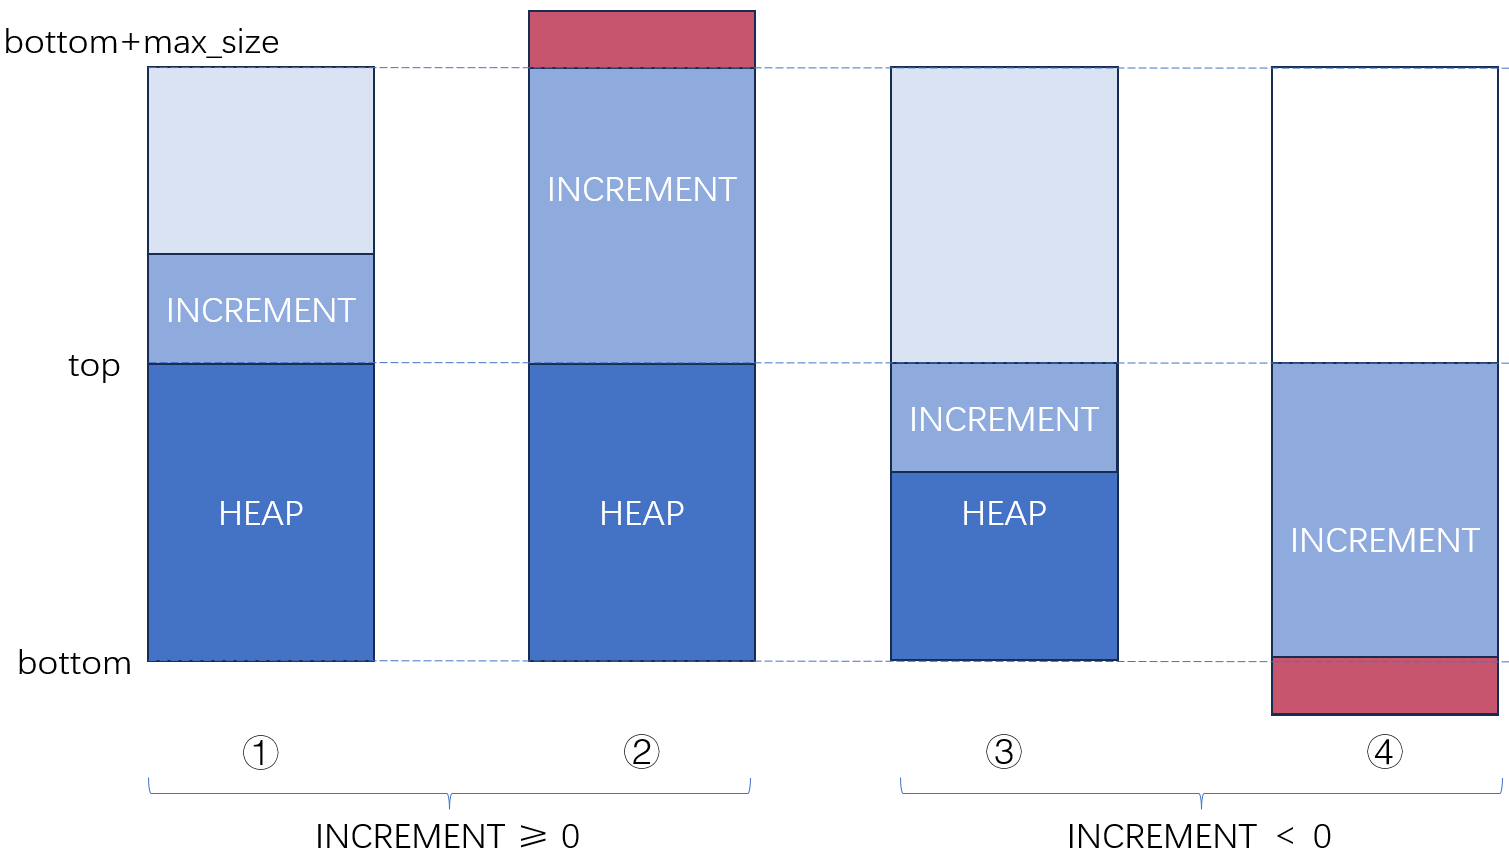
\includegraphics[width=\textwidth]{figures/03-01-使用sbrk四种情况.png}
    \caption{
        使用sbrk四种情况
    }
    \label{fig:使用sbrk四种情况}
\end{figure}

前两种情况代表堆空间的扩大,后两种情况代表堆空间的缩小。有两种可能遇到的问题:
一是堆空间扩大时超过用户空间大小限制;二是堆空间缩小时堆顶指针小于堆底指针。
这两种情况都是不合理的请求时,我们来编写用户态程序测试一下。

\begin{lstlisting}[language={Rust}, label={code:sbrk_test},
    caption={sbrk_test}]
user_lib::println!("old_heap_pt:{:08x}", sbrk(0));
user_lib::println!("increment:8192, 	new_heap_pt:{:08x}", sbrk(8192));
user_lib::println!("increment:-4096, 	new_heap_pt:{:08x}", sbrk(-4096));
user_lib::println!("increment:99999999, 	new_heap_pt:{:08x}", sbrk(99999999));
user_lib::println!("increment:-8192, 	new_heap_pt:{:08x}", sbrk(-8192));
\end{lstlisting}

运行结果如\autoref{fig:使用sbrk四种情况运行截图}:

\begin{figure}[htb]
    \centering
    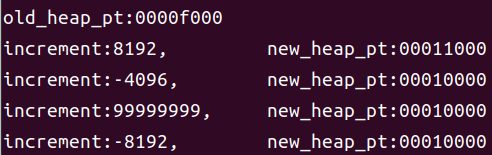
\includegraphics[width=\textwidth]{figures/03-01-使用sbrk四种情况运行截图.png}
    \caption{
        使用sbrk四种情况运行截图
    }
    \label{fig:使用sbrk四种情况运行截图}
\end{figure}

进程的堆空间初始时堆顶指针为0x0f00,语句二调用了sbrk函数,为堆空间增大了8KiB空间,
因此堆顶指针为0x0f00+0x0200=0x1100。同理,语句三缩小了堆空间,也能够正常执行。
第三、四条语句展示了申请的堆空间过大/过小的情况,可见面对这两种错误,sbrk函数选择不改变原来的堆空间。